% Prezentare Scheduler folosind LaTeX Beamer
\documentclass[aspectratio=169]{beamer}
\usepackage[utf8]{inputenc}
\usepackage[T1]{fontenc}
\usepackage{lmodern}
\usepackage{amsmath}
\usepackage{amsfonts}
\usepackage{amssymb}
\usepackage{graphicx}
\usepackage{xcolor}
\usepackage{booktabs}
\usepackage{hyperref}
\usepackage{tikz}

% Culori și tema
\usetheme{Madrid}
\usecolortheme{dolphin}
\setbeamertemplate{navigation symbols}{}
\setbeamertemplate{footline}[frame number]

% Informatii
\title{Scheduler - Planificator de Sarcini Automate}
\subtitle{Proiect de Licență}
\author{Pop Bogdan}
\institute{Universitatea Tehnică din Cluj-Napoca\\Centrul Universitar Nord Baia Mare\\Facultatea de Matematică și Informatică}
\date{\today}

\begin{document}

% Slide de titlu
\begin{frame}
  \titlepage
\end{frame}

% Cuprins
\begin{frame}{Cuprins}
  \tableofcontents
\end{frame}

\section{Rezumat Executiv}
\begin{frame}{Rezumat Executiv}
  \begin{itemize}
    \item Instrument de planificare automatizată a sarcinilor cu:
    \begin{itemize}
      \item planificarea sarcinilor unice sau recurente în format cron
      \item interfață text interactivă ușor de utilizat
      \item notificări desktop pentru finalizarea sau eșecul sarcinilor
      \item persistența sarcinilor între reporniri
      \item funcționează ca serviciu daemon de sistem
    \end{itemize}
    \item Scop: automatizarea și optimizarea executării sarcinilor repetitive, crescând productivitatea utilizatorilor
  \end{itemize}
\end{frame}

\section{Tema și Motivația}
\begin{frame}{Tema și Motivația}
  \begin{columns}
    \begin{column}{0.5\textwidth}
      \textbf{Provocări:}
      \begin{itemize}
        \item executarea manuală a sarcinilor repetitive consumă timp
        \item nevoia de a rula sarcini la intervale specifice
        \item lipsa unei interfețe simple pentru planificarea sarcinilor
        \item necesitatea urmăririi și logării executării sarcinilor
      \end{itemize}
    \end{column}
    \begin{column}{0.5\textwidth}
      \textbf{Motivație:}
      \begin{itemize}
        \item automatizarea sarcinilor repetitive
        \item programarea flexibilă a sarcinilor
        \item monitorizare și notificări pentru starea sarcinilor
        \item persistența sarcinilor între reporniri sistem
      \end{itemize}
    \end{column}
  \end{columns}
\end{frame}

\section{Analiză Comparativă}
\begin{frame}{Analiză Comparativă}
  \begin{tabular}{p{0.3\textwidth} p{0.6\textwidth}}
    \toprule
    \textbf{Soluție} & \textbf{Caracteristici} \\
    \midrule
    Cron (Linux) & planificare puternică, dar fără interfață prietenoasă și fără notificări \\
    \hline
    Task Scheduler (Windows) & interfață grafică, lipsă format cron, complexitate ridicată \\
    \hline
    Alte soluții & fie prea complexe, fie cu funcționalitate limitată \\
    \hline
    \textbf{Soluția propusă} & combină ușurința utilizării cu flexibilitatea programării cron și notificări desktop \\
    \bottomrule
  \end{tabular}
\end{frame}

\section{Soluție Propusă}
\begin{frame}{Soluție Propusă}
  \textbf{Planificator de sarcini bazat pe Python:}
  \begin{itemize}
    \item Interfață text interactivă pentru adăugare, listare și eliminare sarcini
    \item Suport pentru formate cron și programare la dată/oră specifică:
    \begin{itemize}
      \item \texttt{*/15 * * * *} - La fiecare 15 minute
      \item \texttt{0 0 * * *} - În fiecare zi la miezul nopții
    \end{itemize}
    \item Persistența sarcinilor în fișiere JSON
    \item Notificări desktop pentru monitorizarea sarcinilor
    \item Funcționare ca serviciu daemon în fundal
  \end{itemize}
\end{frame}

\section{Opțiuni Tehnice}
\begin{frame}{Opțiuni Tehnice}
  \begin{columns}
    \begin{column}{0.5\textwidth}
      \textbf{Limbaje:}
      \begin{itemize}
        \item Python 3
      \end{itemize}
      
      \textbf{Framework-uri \& API-uri:}
      \begin{itemize}
        \item APScheduler
        \item Plyer
        \item Python-daemon
      \end{itemize}
    \end{column}
    \begin{column}{0.5\textwidth}
      \textbf{Instrumente:}
      \begin{itemize}
        \item JSON pentru stocarea datelor
        \item Systemd pentru servicii sistem
        \item Logging pentru monitorizare
      \end{itemize}
    \end{column}
  \end{columns}
\end{frame}

\section{Fluxul Aplicației}
\begin{frame}{Fluxul Aplicației}
  \begin{enumerate}
    \item \textbf{Inițializare:} încărcare sarcini anterioare din fișier JSON
    \item \textbf{Interfața meniu:} navigare prin opțiuni (adăugare, listare, eliminare sarcini)
    \item \textbf{Adăugare sarcină:} specificare ID, comandă, frecvență (cron/one-time)
    \item \textbf{Execuție sarcină:} rulare comandă, captare rezultat, notificare
    \item \textbf{Persistență:} salvare automată a sarcinilor în JSON după modificări
  \end{enumerate}
  
  \begin{center}
    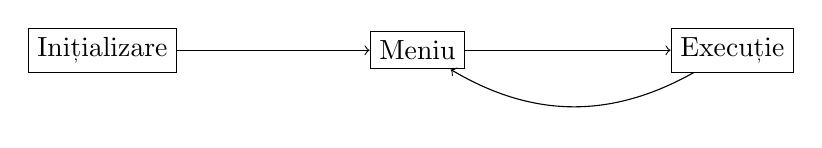
\begin{tikzpicture}[node distance=2cm]
      \node (init) [draw, rectangle] {Inițializare};
      \node (menu) [draw, rectangle, right of=init, xshift=2cm] {Meniu};
      \node (exec) [draw, rectangle, right of=menu, xshift=2cm] {Execuție};
      
      \draw[->] (init) -- (menu);
      \draw[->] (menu) -- (exec);
      \draw[->] (exec) edge[bend left] (menu);
    \end{tikzpicture}
  \end{center}
\end{frame}

\section{Concluzii \& Pași Următori}
\begin{frame}{Concluzii \& Pași Următori}
  \begin{columns}
    \begin{column}{0.5\textwidth}
      \textbf{Concluzii:}
      \begin{itemize}
        \item automatizare eficientă a sarcinilor repetitive
        \item interfață intuitivă și flexibilă
        \item monitorizare fiabilă a statusului sarcinilor
      \end{itemize}
    \end{column}
    \begin{column}{0.5\textwidth}
      \textbf{Pași următori:}
      \begin{itemize}
        \item implementarea unei interfețe grafice
        \item extinderea opțiunilor de programare
        \item adăugarea sistemului de dependențe între sarcini
        \item implementarea unui sistem de failover și backup
      \end{itemize}
    \end{column}
  \end{columns}
\end{frame}

\section{Referințe}
\begin{frame}{Referințe}
  \begin{itemize}
    \item \url{https://apscheduler.readthedocs.io/}
    \item \url{https://plyer.readthedocs.io/}
    \item \url{https://pypi.org/project/python-daemon/}
    \item \url{https://www.freedesktop.org/software/systemd/man/systemd.service.html}
    \item \url{https://docs.python.org/3/library/logging.html}
  \end{itemize}
\end{frame}

\end{document} 